%% Copyright 2026 The ScaleNative Authors.
%% All rights reserved.  Not under the repository's Apache-2.0 license; see ../README.md.
%%
%% fig-layout.tex -- post-route layout of one PE: the base image fig-layout-base.png with the frames, leaders
%% and names drawn over it.  One PDF page of 3.33 in x 3.33 in; the whole page is the die.
%% The base image is drawn by a script from the routed design data; it is not a screenshot of a layout tool.
%% The script and the data are not in this repository (see README.md).  Coordinates are TeX points on the page.
\documentclass[border=0pt]{standalone}
\usepackage[T1]{fontenc}
\usepackage{graphicx}
\usepackage{tikz}
\pdfinfoomitdate=1 \pdfsuppressptexinfo=-1 \pdftrailerid{} \pdfinfo{/Producer (pdfTeX) /Creator (TeX)}
\newcommand{\FigFont}[2]{\fontencoding{T1}\fontfamily{qhv}\fontseries{#1}\fontshape{n}\fontsize{#2bp}{#2bp}\selectfont}
\begin{document}%
\begin{tikzpicture}[x=1pt,y=1pt,line cap=butt,line join=miter]
\useasboundingbox (0,0) rectangle (240.6591,240.6591);
\node[anchor=south west,inner sep=0pt,outer sep=0pt] at (0,0) {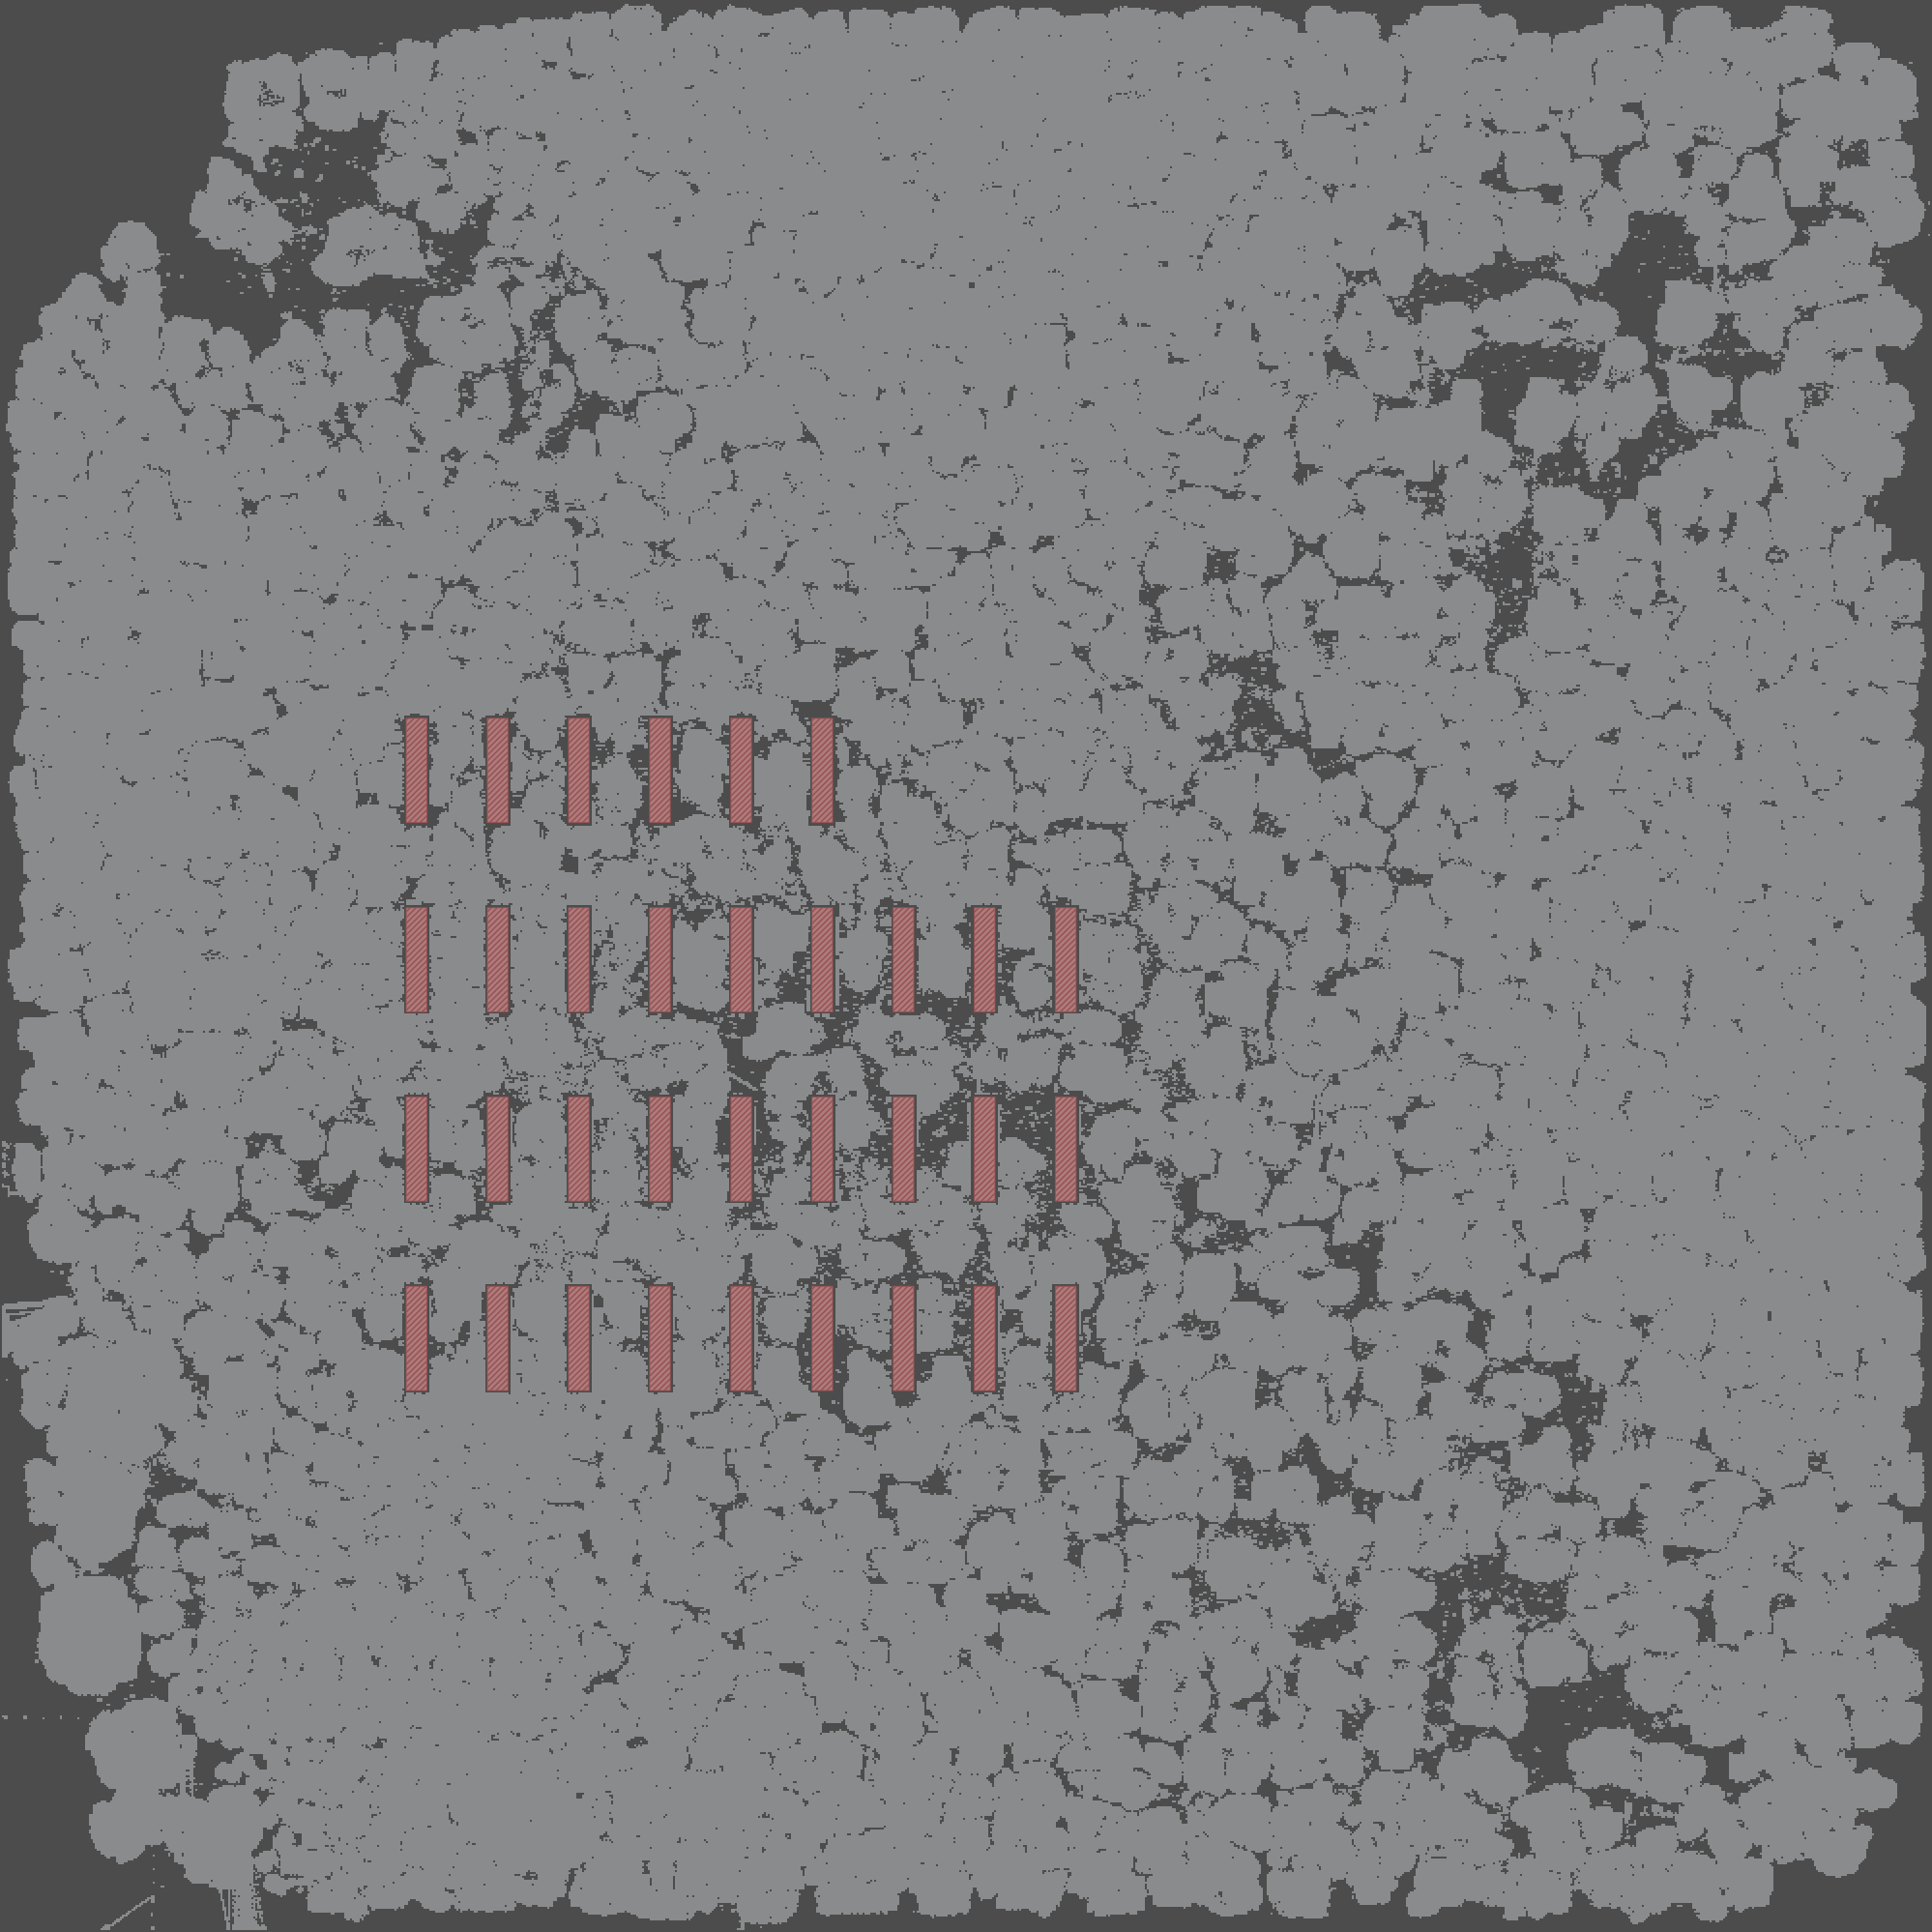
\includegraphics[width=240.6591pt,height=240.6591pt]{fig-layout-base.png}};
\clip (0,0) rectangle (240.6591,240.6591);
\draw[line width=1bp] (0.5019,0.5019) rectangle (240.1572,240.1572);% die outline, drawn just inside the page
\draw[line width=1bp] (5.0541,28.6397) -- (16.8469,28.6397) -- (16.8469,52.2253) -- (20.2163,52.2253) -- (20.2163,69.0722) -- (6.7388,69.0722) -- (6.7388,52.2253) -- (5.0541,52.2253) -- cycle;%% frame: Command processor
\draw[line width=1bp] (10.1081,0.0000) -- (32.0091,0.0000) -- (32.0091,18.5316) -- (23.5856,18.5316) -- (23.5856,28.6397) -- (10.1081,28.6397) -- cycle;%% frame: Ibex CPU
\draw[line width=1bp] (32.0091,0.0000) -- (102.7660,0.0000) -- (102.7660,35.3785) -- (72.4416,35.3785) -- (72.4416,62.3335) -- (20.2163,62.3335) -- (20.2163,52.2253) -- (16.8469,52.2253) -- (16.8469,28.6397) -- (23.5856,28.6397) -- (23.5856,18.5316) -- (32.0091,18.5316) -- cycle;%% frame: Vector unit
\draw[line width=1bp] (97.3745,62.3335) -- (138.1445,62.3335) -- (138.1445,109.3139) -- (77.1572,109.3139) -- (77.1572,132.8982) -- (47.1713,132.8982) -- (47.1713,85.7296) -- (97.3745,85.7296) -- cycle;%% frame: L2
\draw[line width=1bp] (47.1713,62.3335) -- (97.3745,62.3335) -- (97.3745,85.7296) -- (47.1713,85.7296) -- cycle;%% frame: L1
\draw[line width=1bp] (77.1572,109.3139) -- (138.1445,109.3139) -- (138.1445,132.8982) -- (107.4816,132.8982) -- (107.4816,156.6760) -- (47.1713,156.6760) -- (47.1713,132.8982) -- (77.1572,132.8982) -- cycle;%% frame: Operand buffer
\draw[line width=0.7bp] (87.2669,58.8799) -- (87.2669,71.5993); \fill (87.2669,71.5993) circle[radius=1.2bp];% leader: L1
\draw[line width=0.7bp] (77.1587,160.5508) -- (77.1587,146.5679); \fill (77.1587,146.5679) circle[radius=1.2bp];% leader: Operand buffer
\draw[line width=0.7bp] (23.2487,45.8235) -- (11.7928,45.8235); \fill (11.7928,45.8235) circle[radius=1.2bp];% leader: Command processor
\draw[line width=0.7bp] (32.7672,9.0131) -- (25.2703,9.0131); \fill (25.2703,9.0131) circle[radius=1.2bp];% leader: Ibex CPU
\node[anchor=base west,inner sep=0pt,outer sep=0pt] at (152.9449,170.8262) {\FigFont{b}{12}Tensor unit};
\node[anchor=base west,inner sep=0pt,outer sep=0pt] at (36.2633,20.8890) {\FigFont{b}{12}Vector unit};
\node[anchor=base west,inner sep=0pt,outer sep=0pt] at (56.8938,106.0279) {\FigFont{b}{9}L2};
\node[anchor=base west,inner sep=0pt,outer sep=0pt] at (81.9957,50.2871) {\FigFont{b}{9}L1};
\node[anchor=base west,inner sep=0pt,outer sep=0pt] at (44.8103,163.4982) {\FigFont{b}{9}Operand buffer};
\node[anchor=base west,inner sep=0pt,outer sep=0pt] at (25.2703,48.8560) {\FigFont{b}{9}Command};
\node[anchor=base west,inner sep=0pt,outer sep=0pt] at (25.2703,38.1058) {\FigFont{b}{9}processor};
\node[anchor=base west,inner sep=0pt,outer sep=0pt] at (34.7046,5.7279) {\FigFont{b}{9}Ibex CPU};
\end{tikzpicture}%
\end{document}
